\hypertarget{communications_8h}{
\section{/Users/nikki/nublabs/nub.datalogger/hardware/temperature\_\-sensor\_\-Terciopelo/communications.h File Reference}
\label{communications_8h}\index{/Users/nikki/nublabs/nub.datalogger/hardware/temperature\_\-sensor\_\-Terciopelo/communications.h@{/Users/nikki/nublabs/nub.datalogger/hardware/temperature\_\-sensor\_\-Terciopelo/communications.h}}
}
{\tt \#include $<$HardwareSerial.h$>$}\par
{\tt \#include $<$string.h$>$}\par


Include dependency graph for communications.h:\nopagebreak
\begin{figure}[H]
\begin{center}
\leavevmode
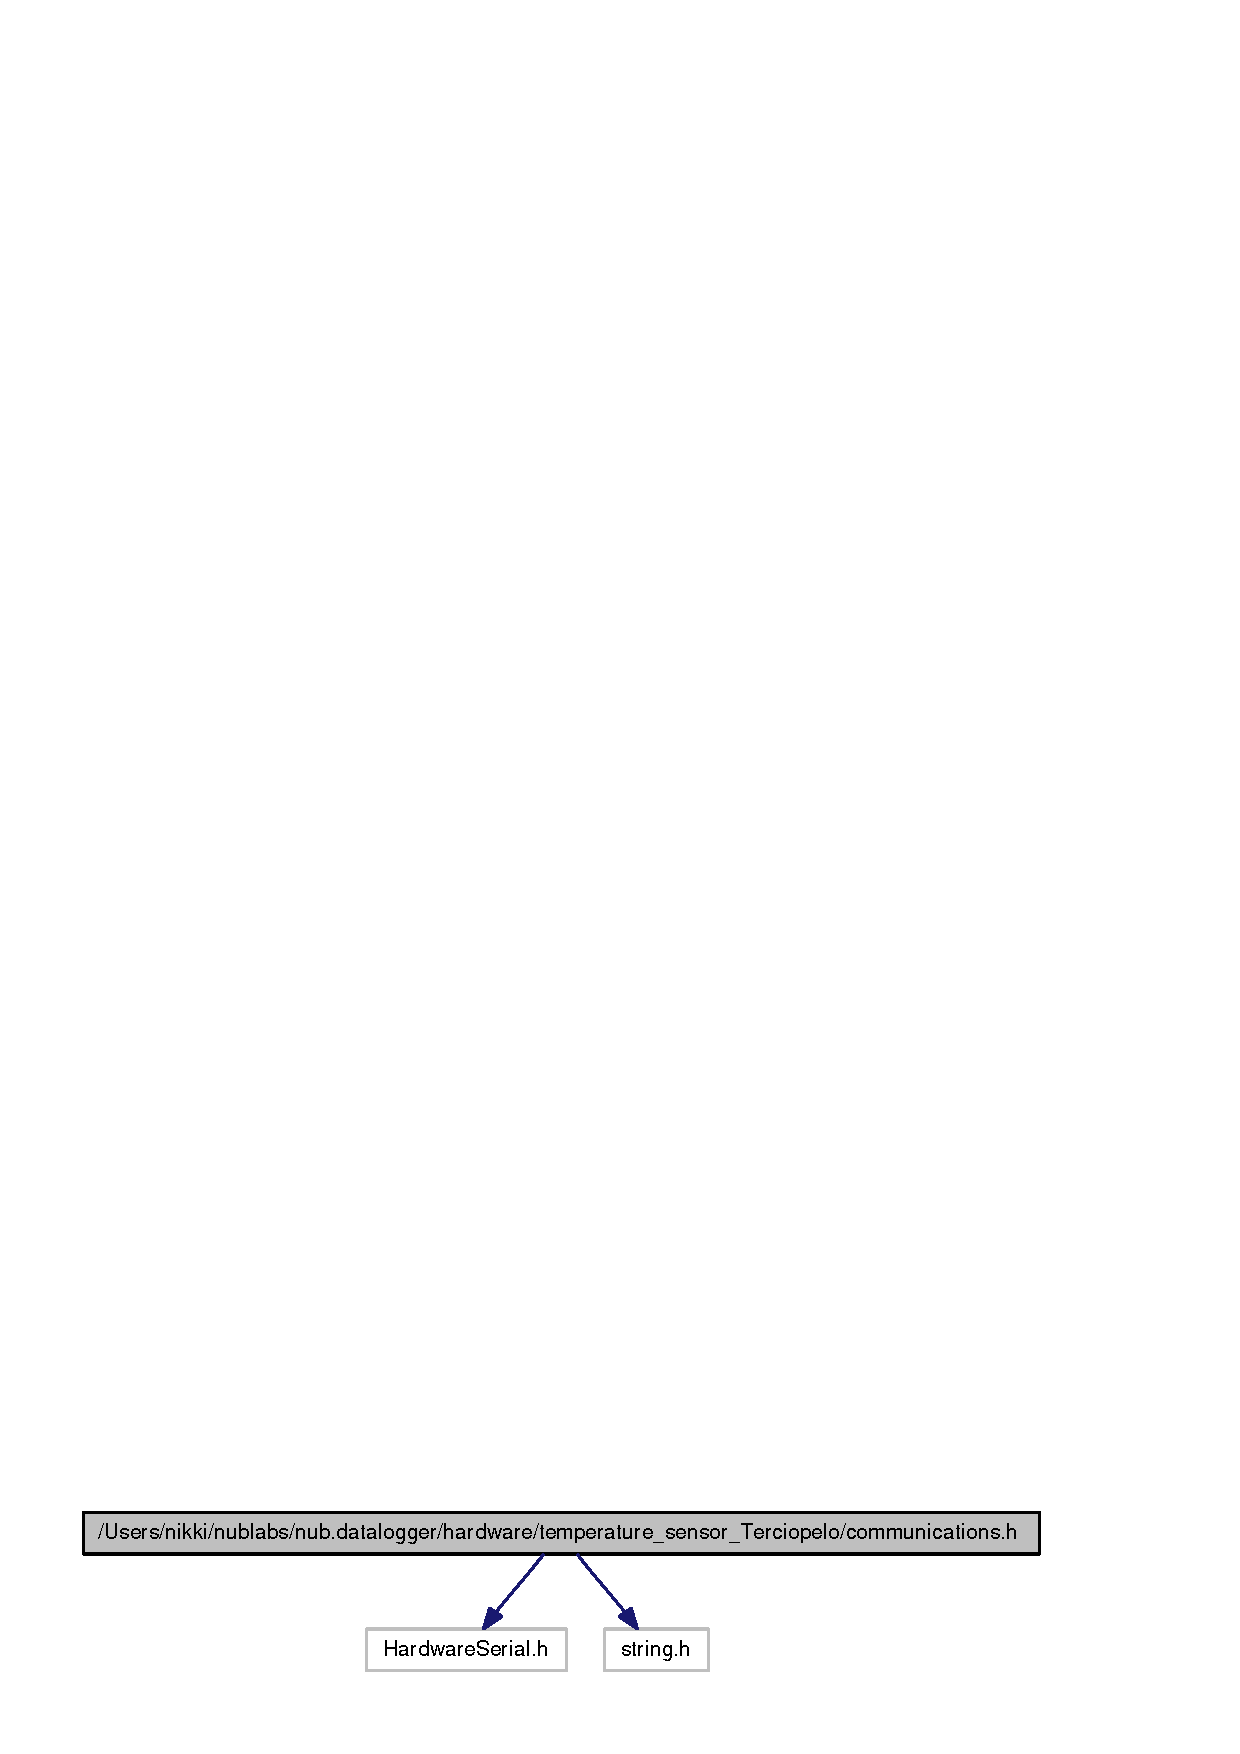
\includegraphics[width=251pt]{communications_8h__incl}
\end{center}
\end{figure}


This graph shows which files directly or indirectly include this file:\nopagebreak
\begin{figure}[H]
\begin{center}
\leavevmode
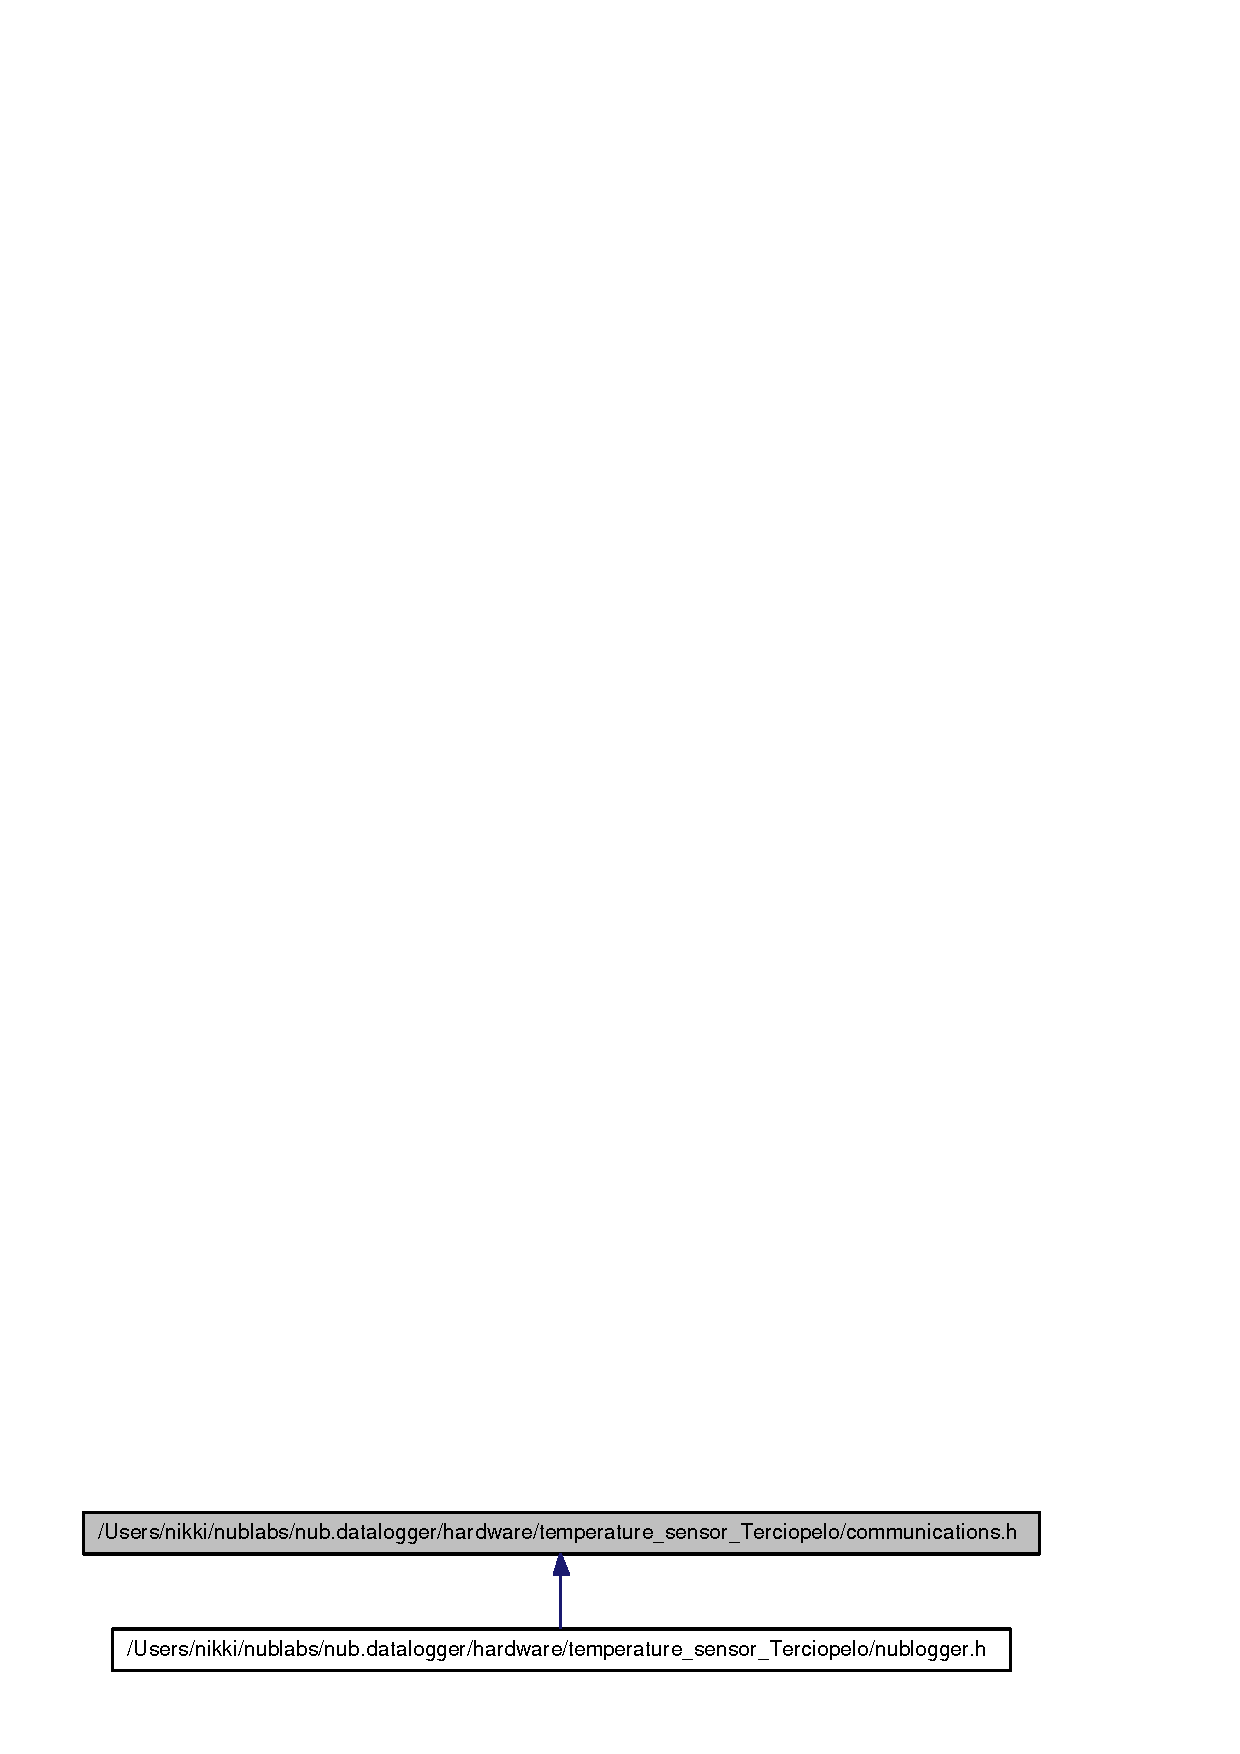
\includegraphics[width=251pt]{communications_8h__dep__incl}
\end{center}
\end{figure}
\subsection*{Functions}
\begin{CompactItemize}
\item 
int \hyperlink{communications_8h_f8c68e93feeba5b9244094043672bac0}{getByte} (int timeout)
\end{CompactItemize}


\subsection{Function Documentation}
\hypertarget{communications_8h_f8c68e93feeba5b9244094043672bac0}{
\index{communications.h@{communications.h}!getByte@{getByte}}
\index{getByte@{getByte}!communications.h@{communications.h}}
\subsubsection[{getByte}]{\setlength{\rightskip}{0pt plus 5cm}int getByte (int {\em timeout})}}
\label{communications_8h_f8c68e93feeba5b9244094043672bac0}




Definition at line 4 of file communications.h.

\begin{Code}\begin{verbatim}5 {
6   int currentTime=millis();
7   int maxTime=currentTime+timeout;
8   while((Serial.available()==0)&&(millis()<(maxTime)))
9     {}
10   if((millis()>maxTime)||(Serial.available()==0))
11     return -1;
12   else
13     return Serial.read();
14 }
\end{verbatim}
\end{Code}


